\section{Experimentación}

    En esta sección, se presentan las pruebas experimentales que se realizaron, junto con los resultados obtenidos y una discusión de los mismos.

    En primer lugar, se detallan las experiencias relacionadas con el método de \emph{PageRank} y su aplicación en el desarrollo de motores de búsqueda. Estos experimentos se hallan orientados a evaluar, por un lado, el rendimiento y la convergencia del otro, y por otra parte, la calidad de los resultados obtenidos.

    A continuación, se encuentran las pruebas relacionadas con respecto al método \emph{GeM}. Estas se encuentran focalizadas en la elaboración de \emph{rankings} para ligas futbolísticas, estudiando la factibilidad de la aplicación del algoritmo en este contexto particular, y diversas alternativas para resolver la dificultad que se presenta a la hora de tener en cuenta los empates.

    Cabe señalar que con los archivos fuente del trabajo práctico se incluye una serie de scripts, en lenguajes Bash y Python, que permiten reproducir por completo los experimentos realizados, como así también los gráficos que se incluyen en este informe. Estos se encuentran dentro del directorio \texttt{exp}, y llevan los nombres \texttt{exp{i}.sh}, siendo \texttt{i} el número de experimento.

    \subsection{Experimentación sobre \emph{PageRank} y páginas web}

        \subsubsection{Experimento 1: Tiempo de ejecución de \emph{PageRank}}

            \subsubsection*{Presentación}
                El objetivo de este experimento fue extraer conclusiones acerca de la variación en el tiempo de cómputo requerido por el algoritmo de \emph{PageRank} para redes de diferentes tamaños, en función de la cantidad de páginas y de la cantidad de \emph{links} de las mismas.

            \subsubsection*{Metodología, datos y parámetros del experimento}
                Se realizaron pruebas para medir el rendimiento temporal según dos parámetros:
                \begin{enumerate}[label=(\alph*)]
                    \item Cantidad de páginas de la red. Se consideraron redes generadas artificialmente con las siguientes cantidades de nodos: \{400, 600, 800, 1000, 1200, 1400, 1600, 1800, 2000, 4000, 6000, 8000, 10000, 20000, 40000, 60000, 80000, 100000\}, estableciendo en todas ellas la misma cantidad de enlaces, 100000.

                    \item Cantidad de enlaces de la red. Se consideraron redes generadas artificialmente con una cantidad fija de 1050 nodos, variando la cantidad de enlaces establecidos entre ellos, tomando los valores \{1000, 5000, 10000, 20000, 40000, 60000, 80000, 100000, 150000, 200000, 300000, 400000, 500000, 600000, 800000, 1000000\}.
                \end{enumerate}

                En todos los casos, para la generación de las instancias de prueba, se distribuyó uniformemente entre las páginas la cantidad de \emph{links} salientes; las páginas hacia los que estos apuntan fueron determinadas al azar.

                El parámetro de amortiguación $c$ se mantuvo fijo con el valor 0.85 (el utilizado normalmente por el buscador Google\cite{Brin1998}), mientras que el umbral de tolerancia para la detención del método se fijó en 0.001.

                En cada caso, se midió el tiempo necesario para la construcción de la matriz que modela la red y para la ejecución de todas las iteraciones necesarias del método. Para realizar las mediciones se utilizaron las funciones provistas a tal efecto por la biblioteca estándar de C++. Con el fin de evitar posibles errores en las mismas, cada una se repitió 20 veces, considerando luego el promedio entre los valores obtenidos.

            \subsubsection*{Hipótesis}
            Es importante considerar en este punto la forma en que la implementación del algoritmo \emph{PageRank} aprovecha la propiedad de la matriz que modela la red ($\mat{P_1}$) de ser esparsa. Una inspección al código de dicha implementación revela que la única operación costosa que se realiza en cada iteración es  el producto entre la dicha matriz y el vector resultante de la iteración anterior. Dentro de este producto existen dos ciclos no anidados; uno de ellos itera sobre todas las posiciones no nulas de la matriz, es decir, linealmente en la cantidad de \emph{links} de la red, para realizar el producto del vector con estos coeficientes. El otro ciclo se realiza sobre todas las posiciones del vector, cuya cantidad es igual a la cantidad de nodos de la red; cabe destacar que este ciclo es extremadamente simple, consistiendo únicamente en un par de sumas.

            Teniendo en cuenta lo anterior, cabe esperar que el tiempo de ejecución dependa linealmente tanto de la cantidad de nodos de la red como de la cantidad de \emph{links} de la misma, pero con una constante mucho mayor en este último caso.

            \subsubsection*{Resultados obtenidos y discusión}

            \noindent{} \begin{minipage}{\textwidth}
                \begin{center}
                    \vspace{1em}

                    \begin{tabular}{cc}
                        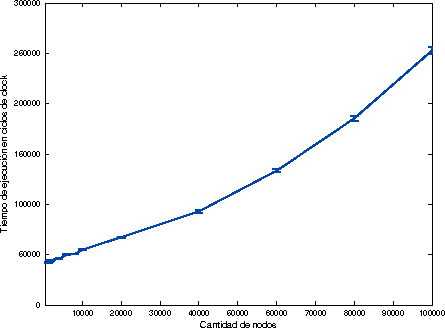
\includegraphics{graficos/exp1-a.pdf} & 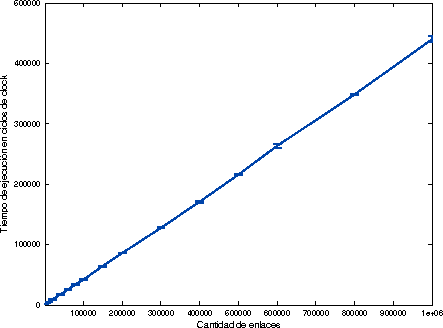
\includegraphics{graficos/exp1-b.pdf} \\
                    \end{tabular}

                    \vspace{1em}

                    Resultados arrojados por el experimento 1. El gráfico de la izquierda representa el tiempo promedio de ejecución del algoritmo \emph{PageRank} en función de la cantidad de nodos de la red, y el de la derecha, en función de la cantidad de \emph{links} de la misma. Se representa también el desvío estándar de las mediciones..

                    \vspace{1em}
                \end{center}
            \end{minipage}

            Como puede observarse en los gráficos que se incluyen, los resultados obtenidos corroboraron la hipótesis de que el tiempo de ejecución del algoritmo aumentaría linealmente con la cantidad de links de la red evaluada. No obstante, la relación con la cantidad de nodos de la red parece no ser lineal, sino de un orden mayor. Aquí entra en juego, muy probablemente, un hecho que no fue tomado en cuenta al elaborar las hipótesis: la naturaleza iterativa del método, que no permite determinar cuántas veces se ejecutará hasta detenerse a partir de una simple inspección de los ciclos del algoritmo. Es decir, hay que tener en cuenta que un incremento en la cantidad de nodos de la red puede tener un efecto no solo en la complejidad de cada iteración particular, sino en la cantidad total de iteraciones requeridas para alcanzar un resultado.

            En efecto, al considerarse una red con más nodos, los valores del vector que se espera obtener luego de cada iteración disminuyen en magnitud, ya que siempre deben sumar 1, al tiempo que aumenta su cantidad. La evidencia empírica obtenida parece indicar que este incremento progresivo del tamaño de la red causó efectos en el cálculo de la norma Manhattan entre los resultados de iteraciones sucesivas, ralentizando la convergencia del algoritmo y alterando el comportamiento que había sido previsto. Este efecto, por otra parte, no parece tener influencia cuando la variable modificada es la cantidad de \emph{links}.

        \subsubsection{Experimento 2: Convergencia de \emph{PageRank}}

            \subsubsection*{Presentación}
            Por medio de este conjunto de pruebas experimentales, se buscó analizar la convergencia lograda por el algoritmo \emph{PageRank} en cada iteración. Como parámetro de la misma, se consideró la diferencia entre el resultado arrojado por dicha iteración y el obtenido en la inmediatamente anterior, en términos de la norma Manhattan de esta diferencia. Teniendo en cuenta que este mismo parámetro es el empleado como criterio de parada del método, se buscó extraer conclusiones sobre la relación entre la tolerancia establecida para dicho criterio y la cantidad de iteraciones necesarias para completar el algoritmo. Además, se analizó la influencia del valor del parámetro $c$ en la convergencia del método.

            \subsubsection*{Metodología, datos y parámetros del experimento}
            A los efectos del experimento, se consideraron las siguientes tres instancias de redes, una de tamaño pequeño y otras dos con cantidad de nodos mayor:
            \begin{enumerate}[label=(\alph*)]
                \item Red pequeña, formada por 50 páginas web reales y la estructura de \emph{links} determinada por las mismas, que al momento del experimento contenía 160 enlaces. La lista de sitios utilizados puede encontrarse en el archivo \texttt{exp/exp2-a-webs.txt}, y el grafo generado, en \texttt{exp/exp2-a-graph.txt}.

                \item Red mediana, formada por las páginas de la Universidad de Stanford (stanford.edu) y los enlaces entre ellas. Comprende 281903 páginas y 2312497 enlaces. Los datos, extraídos de \cite{SNAP}, fueron recopilados en 2002.

                \item Red mediana, formada por las páginas de la Universidad de Notre Dame (nd.edu) y los enlaces entre ellas. Comprende 325729 páginas y 1497134 enlaces. Los datos, extraídos de \cite{SNAP}, fueron recopilados en 1999.
            \end{enumerate}

            Está claro que el tamaño de estas redes no es comparable con el de aquellas que aparecen en el escenario de un buscador web actual (el primer índice de Google, en 1998, contenía 26 millones de páginas \cite{Brin1998}), pero se las consideró suficientes para evaluar el comportamiento del método sin incrementar desmesuradamente los tiempos de ejecución, dejando abierta la posibilidad de realizar, en el futuro, pruebas con instancias mayores.

            Sobre las tres instancias, se ejecutó el algoritmo \emph{PageRank} hasta que la diferencia entre dos iteraciones sucesivas alcanzó el umbral de tolerancia de 0.001 según la norma Manhattan, registrando el valor obtenido para la misma en cada iteración.

            En cuanto al parámetro $c$, el experimento se repitió para cada instancia con los valores \{0.85, 0.90, 0.95, 0.99\}. Se desestimaron valores menores de $c$ porque, como se argumenta en \cite{Kamvar2003}, estos producen resultados poco relevantes y aumentan demasiado la posibilidad de manipulación del método.

            \subsubsection*{Hipótesis}
            Dada la naturaleza iterativa del método, resulta razonable esperar que el ritmo de convergencia del método disminuya a medida que el resultado obtenido se acerca, de forma asintótica, al estado de equilibrio. Esto significa que el costo requerido en cantidad de iteraciones para aumentar la precisión del resultado obtenido se volverá cada vez mayor, apareciendo, en función de los requerimientos específicos del contexto de aplicación, un umbral mínimo para la tolerancia a partir del cual no valdrá la pena continuar ejecutando el método.

            En cuanto al valor de $c$, es importante recordar que valores pequeños de este parámetro determinan, a la hora de construir la matriz $\mat{P_2}$ sobre la que se aplica el algoritmo, un mayor peso relativo de la matriz de amortiguación ($\mat{E}$) con respecto a la que contiene los pesos reales de cada enlace ($\mat{P_1}$). En otras palabras, conforme disminuye el valor de $c$, cabe esperar que la matriz $\mat{P_2}$ sea más homogénea, o que se “se parezca más” a $\mat{E}$.

            Ahora bien, el vector inicial con el que se realiza la primera iteración es un vector homogéneo, que, como puede deducirse fácilmente, es el resultado esperado en caso de que la matriz de la red sea exactamente $\mat{E}$. Por lo tanto, es razonable esperar que ante valores menores de $c$, el vector inicial sea una mejor aproximación del resultado buscado, produciendo que el método converja más rápidamente.

            Por otra parte, los resultados del experimento anterior parecen sugerir que el método tiende a converger más lentamente para redes con más nodos, conjetura que se espera corroborar con las instancias evaluadas en esta prueba. 

            \subsubsection*{Resultados obtenidos y discusión}

            \noindent{} \begin{minipage}{\textwidth}
                \begin{center}
                    \vspace{1em}

                    \begin{tabular}{cc}
                        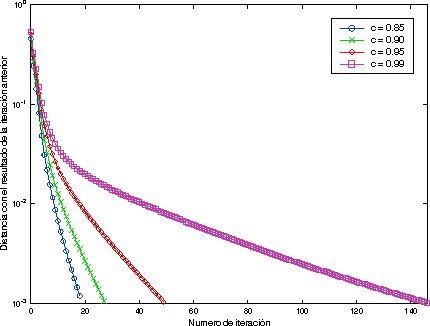
\includegraphics{graficos/exp2-a.pdf} & 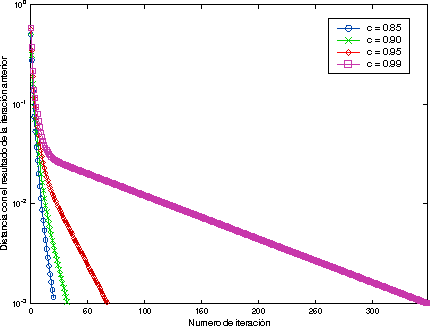
\includegraphics{graficos/exp2-b.pdf} \\
                        {\small Instancia (a)}                & {\small Instancia (b)}
                    \end{tabular}
                \end{center}
            \end{minipage}

            \noindent{} \begin{minipage}{\textwidth}
                \begin{center}
                    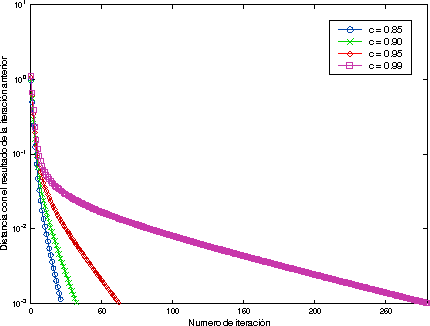
\includegraphics{graficos/exp2-c.pdf} \\
                    {\small Instancia (c)}

                    \vspace{1em}

                    Resultados arrojados por el experimento 2. Los gráficos representan la diferencia Manhattan entre el resultado de cada iteración y el de la inmediatamente anterior durante la ejecución del algoritmo, para las distintas instancias y valores de $c$ considerados.

                    \vspace{1em}
                \end{center}
            \end{minipage}

            La primer conclusión, que resulta evidente de una sencilla observación de los gráficos obtenidos, es que el valor de $c$ tiene, efectivamente, una gran influencia en la convergencia del método: cuando este pasa de 0.95 a 0.99, por ejemplo, la cantidad de iteraciones requeridas para alcanzar el umbral fijado de tolerancia aumenta a casi el triple, en el menos extremo de los tres casos.

            También se corrobora en los gráficos que la convergencia del método es cada vez más lenta conforme avanzan las iteraciones. Se observa, especialmente en el caso de $c = 0.99$, que la convergencia es rápida hasta que se alcanza un punto de inflexión, a partir del cual queda relativamente estancada. Su aproximación a una línea recta en los gráficos, cuyo eje $y$ posee escala logarítmica, sugiere que su comportamiento asintótico es un decrecimiento exponencial.

            Un interesante hecho a notar es que la evidencia empírica contradice la hipótesis de la existencia de una relación inversa entre la cantidad de nodos de la red estudiada y la velocidad de convergencia del método: la instancia (b), pese a poseer considerablemente menos nodos que la instancia (c), requirió para todos los valores estudiados de $c$ una mayor cantidad de iteraciones para alcanzar el umbral de tolerancia aceptado. No es posible, sin embargo, descartar por completo la posibilidad de que tamaño de la red y convergencia estén relacionadas; es necesario tener en cuenta que en el experimento anterior se comparaban redes con la misma cantidad de enlaces y una estructura semejante, características que no poseen las instancias contrastadas en esta prueba, por lo que se considera pendiente para investigaciones futuras la realización de nuevas pruebas donde se estudie la interferencia de estos factores con los resultados observados.

        \subsubsection{Experimento 3: Análisis cualitativo de los resultados}

            \subsubsection*{Presentación}
            Por medio de estas pruebas, se pretende realizar un estudio cualitativo de los resultados arrojados por el método \emph{PageRank}. A modo de contraste, y para realizar una evaluación comparativo, se implementó un método de clasificación alternativo más simple, denominado \textsc{In-deg}. Este consiste en ordenar las páginas considerando simplemente la cantidad de \emph{links} entrantes hacia cada una de ellas. En particular, el puntaje de una página se calcula como el cociente entre la cantidad de enlaces que recibe y el total de los mismos en la red.

            \subsubsection*{Metodología, datos y parámetros del experimento}
            Para esta experiencia se construyeron artificialmente tres redes pequeñas, pensadas con el objetivo de poner de manifiesto y observar las diferencias entre los dos algoritmos planteados. Estos casos de prueba, que ilustra la Figura \ref{fig:exp3-webs}, son los siguientes:
            \begin{enumerate}[label=(\alph*)]
                \item La Web 1 cuenta con ocho nodos. Seis de los mismos (nodos 3 a 8) se encuentran enlazados de forma tal que cada uno de ellos recibe enlaces de exactamente dos de los otros. Uno de los nodos restantes (nodo 1) recibe un enlace de cada uno de estos seis. El otro (nodo 2) recibe solo un enlace de este último.
                \item La Web 2 también posee ocho nodos. Uno de ellos (nodo 1) recibe enlaces de todos los demás. Otro nodo (nodo 2) solo recibe un enlace del nodo 1. El nodo 3 recibe enlaces de los últimos cinco nodos (del 4 al 8). Estos, por su parte, no tienen enlaces entrantes.
                \item La Web 3 se compone de dos subredes no conectadas, una de 4 nodos y otra de 2 nodos. Dentro de ellas, cada nodo recibe exactamente un enlace entrante desde otro nodo.
            \end{enumerate}

            \begin{figure}[h]
                \begin{center}
                    \begin{tabular}{@{\extracolsep{2cm}} cc}
                      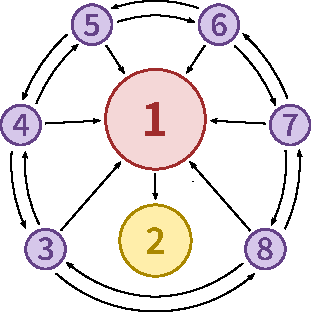
\includegraphics{imagenes/exp3-graph1.pdf} & 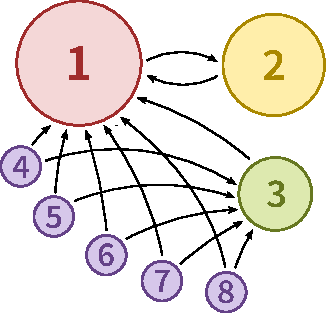
\includegraphics{imagenes/exp3-graph2.pdf} \\
                      {\small \strong{Web 1}} & {\small \strong{Web 2}} \\
                      \multicolumn{2}{c}{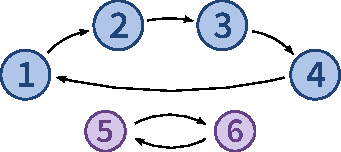
\includegraphics{imagenes/exp3-graph3.pdf}} \\
                      \multicolumn{2}{c}{{\small \strong{Web 3}}} \\
                    \end{tabular}
                \end{center}

                \caption{Redes utilizadas como datos de entrada para el Experimento 3. El tamaño con el que aparece representado cada nodo corresponde al \emph{ranking} que la hipótesis planteada prevé como resultado de \emph{PageRank}.} \label{fig:exp3-webs}
            \end{figure}

            \subsubsection*{Hipótesis}

            Las redes estudiadas pretenden poner de manifiesto las principales características distintivas del algoritmo \emph{PageRank}.

            La primera de ellas presenta un nodo (el nodo 2) que recibe un solo enlace, menos que todos los demás. No obstante, este es un enlace de gran peso, ya que procede del nodo 1, quien recibe a su vez links de todos los nodos restantes. Cabe esperar que esta página sea ignorada por \textsc{In-deg}, pero no por \emph{PageRank}, que seguramente la ubicará por encima de los otros nodos satélites.

            La segunda red presenta un escenario más sutil. Aquí la diferencia se espera entre los nodos 2 y 3: el segundo recibe más enlaces, por lo que será más relevante para \textsc{In-deg}; el primero, sin embargo, recibe un enlace del nodo 1, que ocupa una posición central en la red. Cabe esperar que esto eleve su posición en \emph{PageRank}. También es de interés que el nodo 2 de esta red, a diferencia del de la red anterior, tiene un enlace saliente hacia 1. Dado que esto tiende a incrementar más el puntaje de 1 en \emph{PageRank}, se espera que resulte perjudicial para el puntaje de 2.

            La tercera red es un caso simple de una red no conexa. Para \textsc{In-deg}, todas las páginas tendrán el mismo puntaje, ya que poseen exactamente un \emph{link} entrante. \emph{PageRank}, sin embargo, podría establecer una diferencia a favor de la subred mayor, teniendo en cuenta el \emph{factor de teletransportación}; en caso de ser un navegante aleatorio al momento de teletransportarse, es mayor la probabilidad de moverse a una página de la subred de mayor tamaño.

            \subsubsection*{Resultados obtenidos y discusión}

            \begin{center}
                \begin{tabular}{|c|c|c||c|c|c|}
                    \hline
                    \multicolumn{3}{|c||}{\emph{Ranking} Web 1 - \emph{PageRank}} & \multicolumn{3}{c|}{\emph{Ranking} Web 1 - \textsc{In-deg}} \\ \hline
                    Pos. & Nodo & Puntaje    & Pos. & Nodo & Puntaje  \\ \hline
                    1    & 2    & 0.216403   & 1    & 1    & 0.315789 \\
                    2    & 1    & 0.205549   & 2    & 3    & 0.105263 \\
                    3    & 3    & 0.096341   & 3    & 4    & 0.105263 \\
                    4    & 4    & 0.096341   & 4    & 5    & 0.105263 \\
                    5    & 5    & 0.096341   & 5    & 6    & 0.105263 \\
                    6    & 6    & 0.096341   & 6    & 7    & 0.105263 \\
                    7    & 7    & 0.096341   & 7    & 8    & 0.105263 \\
                    8    & 8    & 0.096341   & 8    & 2    & 0.052632 \\ \hline
                    \multicolumn{6}{c}{} \\ \hline
                    \multicolumn{3}{|c||}{\emph{Ranking} Web 2 - \emph{PageRank}} & \multicolumn{3}{c|}{\emph{Ranking} Web 2 - \textsc{In-deg}} \\ \hline
                    Pos. & Nodo & Puntaje    & Pos. & Nodo & Puntaje  \\ \hline
                    1    & 1    & 0.447829   & 1    & 1    & 0.538462 \\
                    2    & 2    & 0.399828   & 2    & 3    & 0.384615 \\
                    3    & 3    & 0.058594   & 3    & 2    & 0.076923 \\
                    4    & 4    & 0.018750   & 4    & 4    & 0.000000 \\
                    5    & 5    & 0.018750   & 5    & 5    & 0.000000 \\
                    6    & 6    & 0.018750   & 6    & 6    & 0.000000 \\
                    7    & 7    & 0.018750   & 7    & 7    & 0.000000 \\
                    8    & 8    & 0.018750   & 8    & 8    & 0.000000 \\ \hline
                    \multicolumn{6}{c}{} \\ \hline
                    \multicolumn{3}{|c||}{\emph{Ranking} Web 3 - \emph{PageRank}} & \multicolumn{3}{c|}{\emph{Ranking} Web 3 - \textsc{In-deg}} \\ \hline
                    Pos. & Nodo & Puntaje    & Pos. & Nodo & Puntaje  \\ \hline
                    1    & 1    & 0.166667   & 1    & 1    & 0.166667 \\
                    2    & 2    & 0.166667   & 2    & 2    & 0.166667 \\
                    3    & 3    & 0.166667   & 3    & 3    & 0.166667 \\
                    4    & 4    & 0.166667   & 4    & 4    & 0.166667 \\
                    5    & 5    & 0.166667   & 5    & 5    & 0.166667 \\
                    6    & 6    & 0.166667   & 6    & 6    & 0.166667 \\ \hline
                \end{tabular}
            \end{center}

            Los primeros dos casos reflejaron resultados similares a los planteados en la hipótesis, mostrando hasta qué punto \emph{PageRank} tiene en cuenta el peso de los \emph{links} por encima de la cantidad de los mismos. El caso de la Web 1 es especialmente destacable, ya que allí la página 2, que recibe tan solo un enlace, quedó por encima de todas las demás, incluso de la página 1, que recibe 6. \textsc{In-deg}, en cambio, la relegó al último lugar.

            En la Web 2, en cambio, pese a que el escenario es similar, la página 2 quedó en segunda posición. Esto corrobora la hipótesis de que agregar links salientes puede jugar en contra de la posición de una página en el \emph{ranking} de \emph{PageRank}.

            En cuanto a la Web 3, quedó claramente refutada la hipótesis de que las subredes recibirían diferentes puntuaciones de acuerdo a su tamaño. Tanto para \textsc{In-deg} como para \emph{PageRank}, todas las páginas recibieron idéntico puntaje. El escenario de redes no conexas es especialmente interesante por resultar menos intuitivo, y además, porque refleja la estructura real de la Internet, donde se presenta este tipo de subredes. Por lo tanto, profundizar en la experimentación con estos casos es un tema de interés para investigaciones posteriores.

    \subsection{Experimentación sobre \emph{GeM} y ligas deportivas}

        \subsubsection{Experimento 1}
        \subsubsection*{Presentación}
        En este experimento se verá la diferencia entre los métodos de \emph{GeM} y el de la \acr{AFA} para determinar el \emph{ranking} de una liga deportiva. Para ello se tomará como parámetro de entrada una tabla con los partidos, sus respectivas fechas, y sus resultados. En la misma, deberá existir un equipo que ocupe una de las primaras posiciones en la tabla de \emph{rankings} que haya perdido contra otro que ocupa una de las últimas. Observaremos la diferencia entre el \emph{ranking} generado por cada uno de los métodos.

            \subsubsection*{Hipótesis}
            Cuando se juega un partido entre dos equipos, en el método de \emph{GeM} se tendrá en cuenta que tan fuerte son los equipos involucrados y cual fue la diferencia de goles en el partido. En cambio, en el método de la \acr{AFA} el ganador recibirá 3 puntos sin importar los resultados ni las posiciones que los mismos tenían hasta el momento. Esto puede generar diferencias en el \emph{ranking} ya que cada método considera distinta información para determinar las nuevas posiciones.

            Por otro lado, si un equipo que se encuentra en las últimas posiciones de la tabla juega contra uno que está en las primeras y gana, para el método de la \acr{AFA} es exactamente igual que haya jugado con cualquier otro. Para \emph{GeM}, al tener en cuenta que tan fuertes son los equipos, esto generará que el nuevo vencedor quede en una mejor posición en la tabla. Así, en este método, entre dos fechas se pueden generar saltos, es decir, un equipo puede pasar de tener una muy mala posición en la tabla a estar dentro de los mejores solo por haber ganado un partido contra un equipo fuerte. En el método de la \acr{AFA} no pasa ya que sólo se le sumarán 3 puntos al equipo triunfador.

            \subsubsection*{Datos de entrada}
                Resultados del Torneo de Primera División del Fútbol Argentino hasta la Fecha 23. El valor de $c$ es \texttt{0.85} y el valor de tolerancia es \texttt{0.00001}. Se eligió el valor de c y el de la tolerancia arbitrariamente, procurando que los casos de prueba no fueran excesivamente grandes para no prolongar innecesariamente la duración de las pruebas.
.

            \subsubsection*{Resultados}

                \begin{center}
                    \begin{tabular}{|c|c|c||c|c|c|}
                        \hline
                        \multicolumn{3}{|c||}{\emph{Ranking} Liga Deportiva - \emph{GeM}} & \multicolumn{3}{c|}{\emph{Ranking} Liga Deportiva - \acr{AFA}} \\
                        \hline
                        Pos. & Equipo & Puntaje                 & Pos. & Equipo & Puntaje \\ \hline
                        1 & Boca Juniors & 0.080913             & 1 & San Lorenzo & 0.054289 \\
                        2 & Aldosivi & 0.069879                 & 2 & Boca Juniors & 0.053203 \\
                        3 & River Plate & 0.069065              & 3 & Racing Club & 0.049946 \\
                        4 & San Lorenzo & 0.058309              & 4 & Rosario Central & 0.048860 \\
                        5 & San Martín (SJ) & 0.051788          & 5 & River Plate & 0.047774 \\
                        6 & Racing Club & 0.051674              & 6 & Independiente & 0.041260 \\
                        7 & Rosario Central & 0.046326          & 7 & Belgrano & 0.041260 \\
                        8 & Quilmes & 0.045206                  & 8 & Estudiantes (LP) & 0.041260 \\
                        9 & Newell's Old Boys & 0.043581        & 9 & Tigre & 0.040174 \\
                        10 & Vélez Sarsfield & 0.039828         & 10 & Banfield & 0.040174 \\
                        11 & Gimnasia y Esgrima (LP) & 0.035738 & 11 & Lanús & 0.039088 \\
                        12 & Estudiantes (LP) & 0.034629        & 12 & Gimnasia y Esgrima (LP) & 0.038002 \\
                        13 & Belgrano & 0.033908                & 13 & Quilmes & 0.034745 \\
                        14 & Banfield & 0.032996                & 14 & San Martín (SJ) & 0.034745 \\
                        15 & Unión & 0.028015                   & 15 & Unión & 0.033659 \\
                        16 & Defensa y Justicia & 0.027041      & 16 & Tempreley & 0.030402 \\
                        17 & Lanús & 0.026036                   & 17 & Argentinos Juniors & 0.028230 \\
                        18 & Independiente & 0.023666           & 18 & Newell's Old Boys & 0.028230 \\
                        19 & Tigre & 0.023078                   & 19 & Aldosivi & 0.028230 \\
                        20 & Sarmiento & 0.022266               & 20 & Vélez Sarsfield & 0.027144 \\
                        21 & Olimpo & 0.021956                  & 21 & Defensa y Justicia & 0.026059 \\
                        22 & Crucero del Norte & 0.021713       & 22 & Sarmiento & 0.026059 \\
                        23 & Arsenal & 0.018678                 & 23 & Olimpo & 0.024973 \\
                        24 & Argentinos Juniors & 0.017951      & 24 & Colón & 0.024973 \\
                        25 & Tempreley & 0.017670               & 25 & Godoy Cruz & 0.023887 \\
                        26 & Huracán & 0.013740                 & 26 & Huracán & 0.022801 \\
                        27 & Godoy Cruz & 0.013541              & 27 & Atlético de Rafaela & 0.021716 \\
                        28 & Atlético de Rafaela & 0.011738     & 28 & Arsenal & 0.018458 \\
                        29 & Colón & 0.011141                   & 29 & Nueva Chicago & 0.015201 \\
                        30 & Nueva Chicago & 0.007928           & 30 & Crucero del Norte & 0.015201 \\
                        \hline
                    \end{tabular}
                \end{center}

            \subsubsection*{Discusión}

            Como podemos ver en las tablas de \emph{rankings}, los órdenes no son exactamente iguales. Por ejemplo, mirando el equipo 1 (Aldosivi), en el \emph{ranking} de la \acr{AFA} se encuentra en la posición 20 y cuando usamos el método de \emph{GeM} éste está en la posición 2. Esto se debe a que Aldosivi le ganó tanto al equipo 24 (San Lorenzo) como al 7 (Boca Juniors), que se encontraban primero y segundo en la tabla de posiciones de la \acr{AFA}, respectivamente. Por esto, en \emph{GeM} sube muchas posiciones mientras que con la \acr{AFA} sólo se le otorgan 3 puntos por cada uno de los dos partidos.

        \subsubsection{Experimento 2}
            \subsubsection*{Presentación}
            Con este experimento se busca mostrar como varía el ranking de los equipos a medida que van pasando las fechas de la liga para diferentes valores de c. Para ello se tomará la primer fecha y se medirá el ranking hasta el momento. Luego tomaremos la liga completa y se evaluará el ranking final. Esto se repetirá para cada uno de los valores de c. Luego se compararán las variaciones entre el inicio y el fin de la liga para cada uno de los valores.

            \subsubsection*{Hipótesis}
            Suponemos que cuando el grafo es muy poco conexo, es decir, cuando no hay demasiadas conexiones entre los equipos, como es al inicio de la liga, el c cobra relevancia. Por lo tanto, al inicio, para diferentes valores de c va a haber mucha variación en los rankings de los equipos. En cambio, cuando el grafo es mas conexo, es decir, cuando los equipos están muy relacionados entre sí, como sucede al final de la liga, cuando ya se jugaron todas las fechas, la importancia del c disminuye, por lo que suponemos que van a ser muy similares los rankings finales para los diferentes valores de c.

            \subsubsection*{Datos de entrada}
            Se tomará como valor de tolerancia 0.00001 y los valores de c serán 0.2, 0.5 y 0.9. La liga utilizada se encuentra en el archivo matches.txt. Se eligió el valor de la tolerancia arbitrariamente, procurando que los casos de prueba no fueran excesivamente grandes para no prolongar innecesariamente la duración de las pruebas. Los valores de c elegidos son valores intermedios del total de valores que puede tomar (c no puede ser mayor que 1).

            \subsubsection*{Resultados}
            \noindent{} \begin{minipage}{\textwidth}
                \begin{center}
                    \vspace{1em}

                    \begin{tabular}{cc}
                        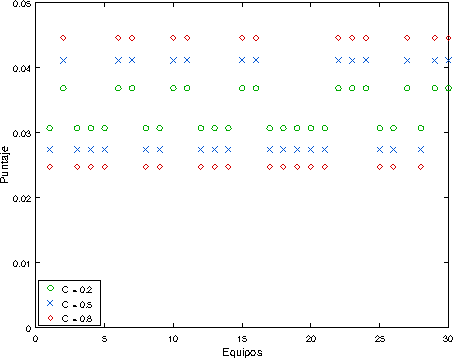
\includegraphics{graficos/exp2-partidos-liga-afa1.pdf} & 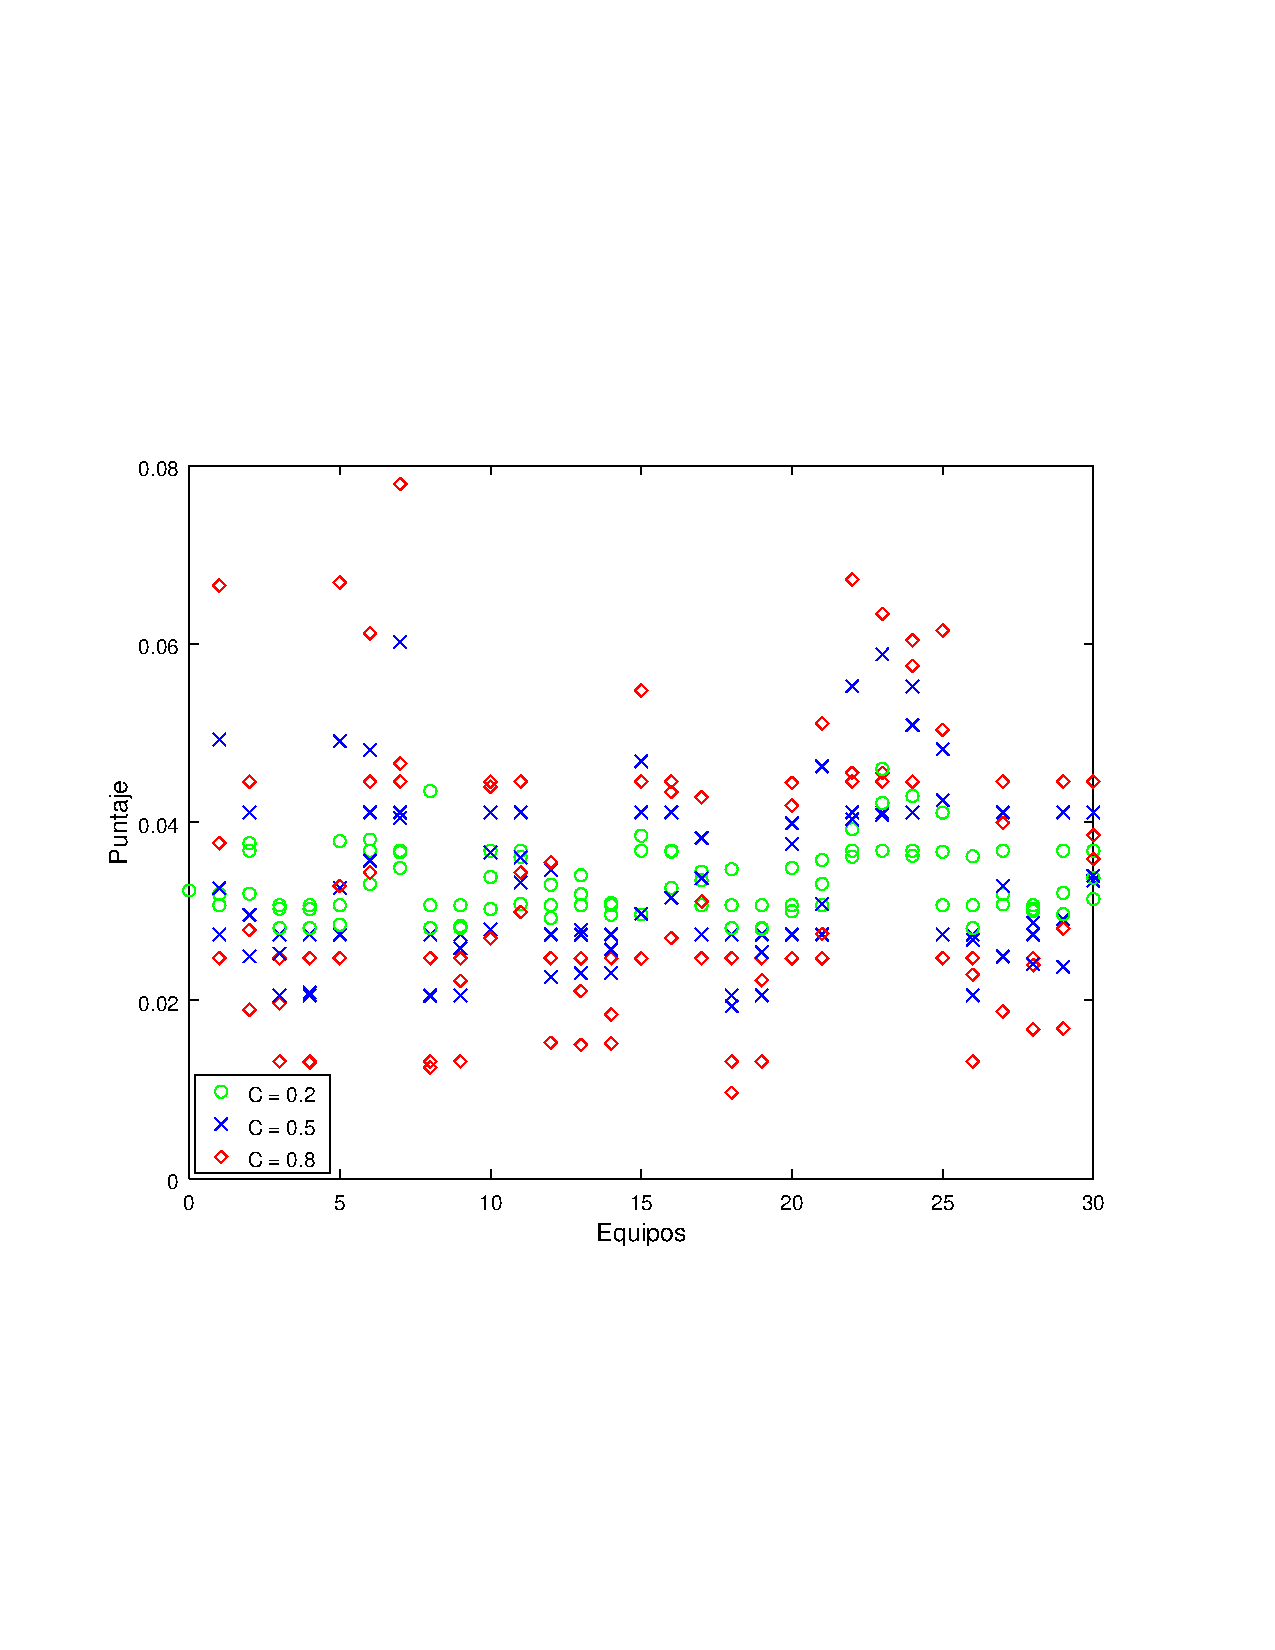
\includegraphics{graficos/exp2-partidos-liga-afa3.pdf} \\
                        {\small 1 fecha}                                       & {\small 5 fechas}
                    \end{tabular}
                \end{center}
            \end{minipage}

            \noindent{} \begin{minipage}{\textwidth}
                \begin{center}
                    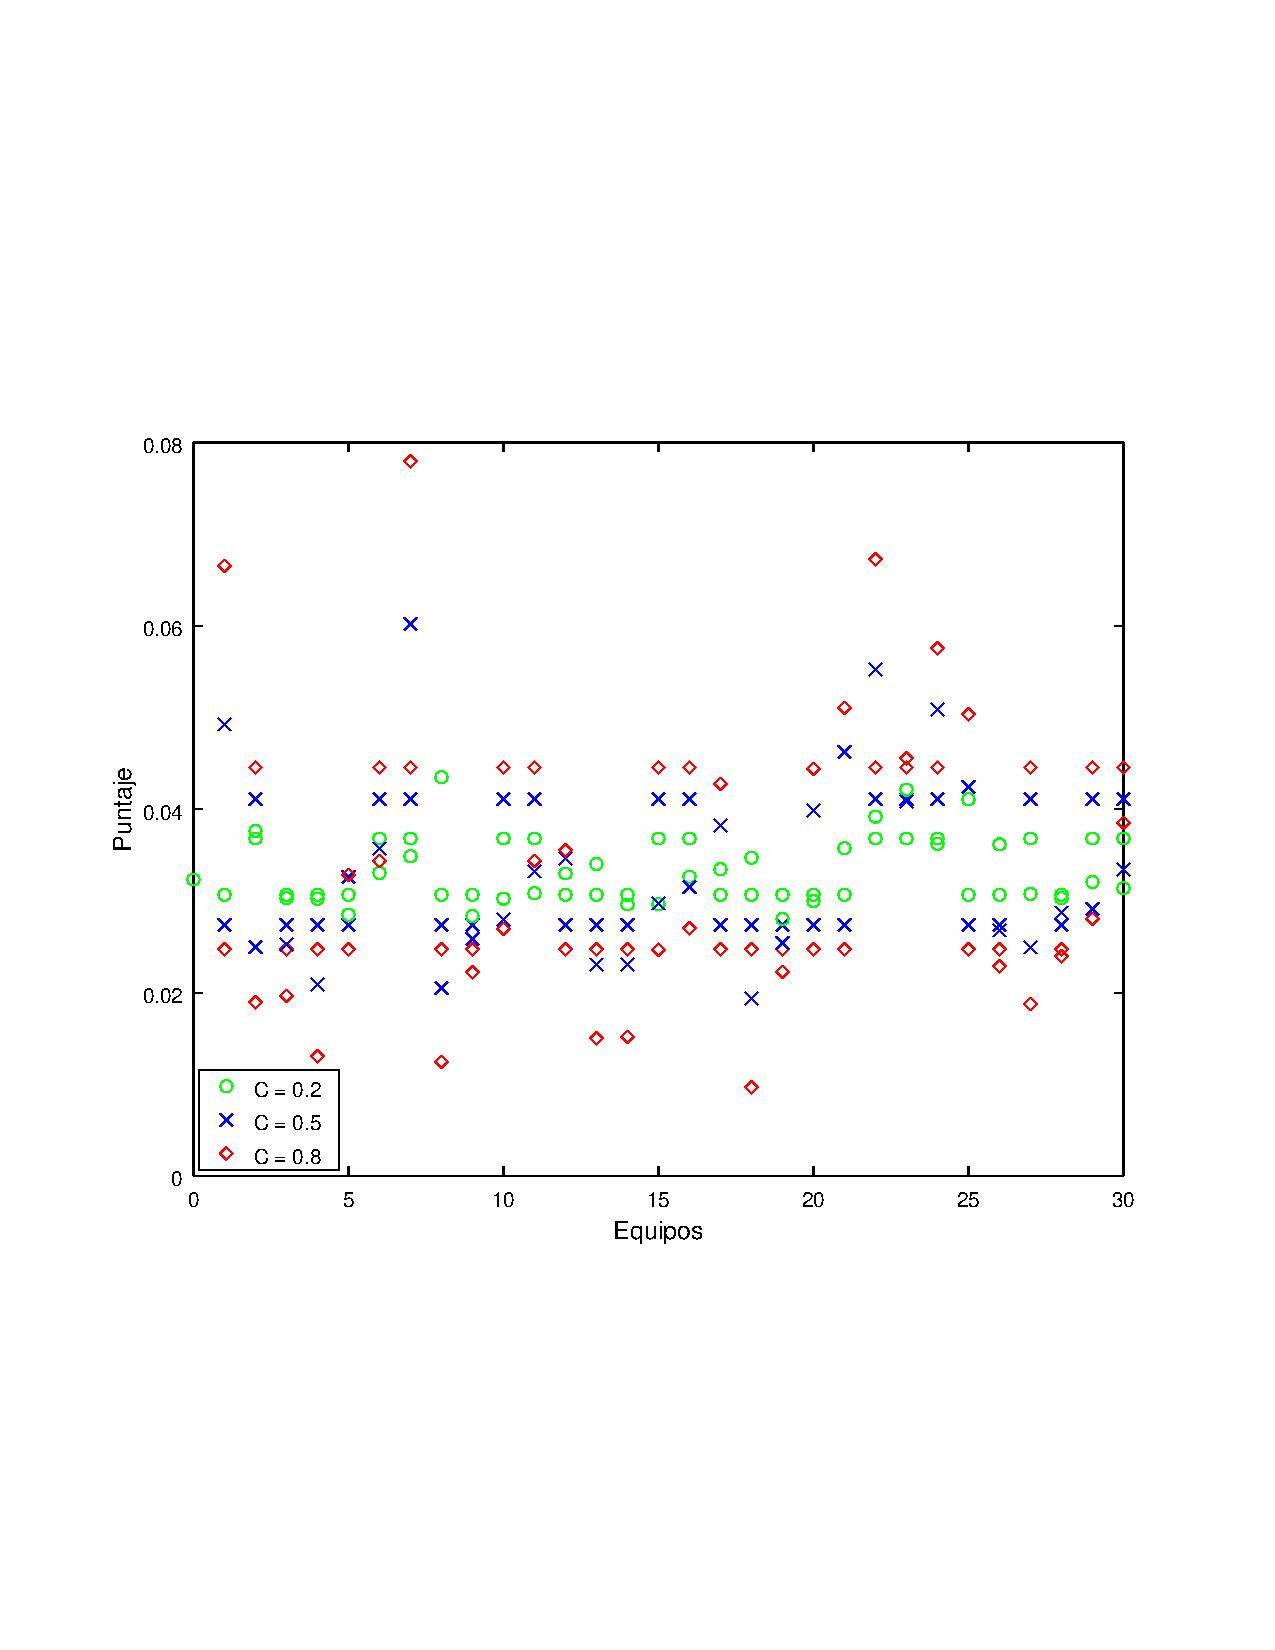
\includegraphics{graficos/exp2-partidos-liga-afa2.pdf} \\
                    {\small 23 fechas}

                    \vspace{1em}

                    Resultados arrojados por el experimento 2. Los gráficos muestran la evolución del \emph{ranking} obtenido mediante \emph{GeM} para la Liga de Primera División de la \acr{AFA}, según el transcurso de las fechas.

                    \vspace{1em}
                \end{center}
            \end{minipage}


            \subsubsection*{Discusión}
            Como se puede observar en los gráficos, en la instancia inicial de la liga los diferentes valores de c generan variaciones mayores entre los puntajes de cada equipo que cuando tomamos el ranking final.
            Además podemos observar que para valores mas chicos de c, los resultados son más homogéneos. Esto se debe a que al decrementar c, incrementamos (1-c) que es la probabilidad de que un equipo juegue con otro y gane. Ésta probabilidad es para todos los equipos igual. Si la aumentamos, entonces ésta tomará más importancia generando así un sistema en el que los puntajes de los diferentes equipos sean mucho mas cercanos.


        \subsubsection{Experimento 3: Casos de empate}

            \subsubsection*{Presentación}
            Cuando dos equipos se enfrentan y empatan, podemos tomar diferentes criterios para asignarles el puntaje correspondiente a ese partido. En este experimento, analizaremos tres posibles métodos de asignación de puntaje. En el primero no se le otorgarán puntos a ninguno de los dos equipos. Es decir, empatar y no haber jugado va a valer lo mismo al momento de medir el ranking final de la liga deportiva. En el segundo de los métodos que se analizará, el puntaje que cada equipo recibirá por haber empatado será pasado por parámetro al momento de armar la tabla de puntuaciones. Éste valor será el mismo para los dos equipos y se denominará $k$.

            El objetivo de este experimento es determinar cual de los tres métodos presentados resuelve mejor la situación del empate. Para ello de tomaron diferentes ligas que constan de 6 equipos que juegan entre si a lo largo de 6 fechas. Cada una de ellas presenta diferentes situaciones de empate.
            En la liga 2 el equipo 1 le gana a todos menos con el 6 que empata. El equipo 6 pierde con todos menos con el 1 que empata. El equipo 2 le gana al 5 y al 3 y pierde con el 4. El 3 le gana al 4 y al 5 y pierde con el 2. El 4 gana contra el 2 y pierde con el 3 y el 5. Por último el 5 gana contra el 4 y pierde contra el 2 y el 3.
                \begin{figure}[h]
                    \begin{center}
                      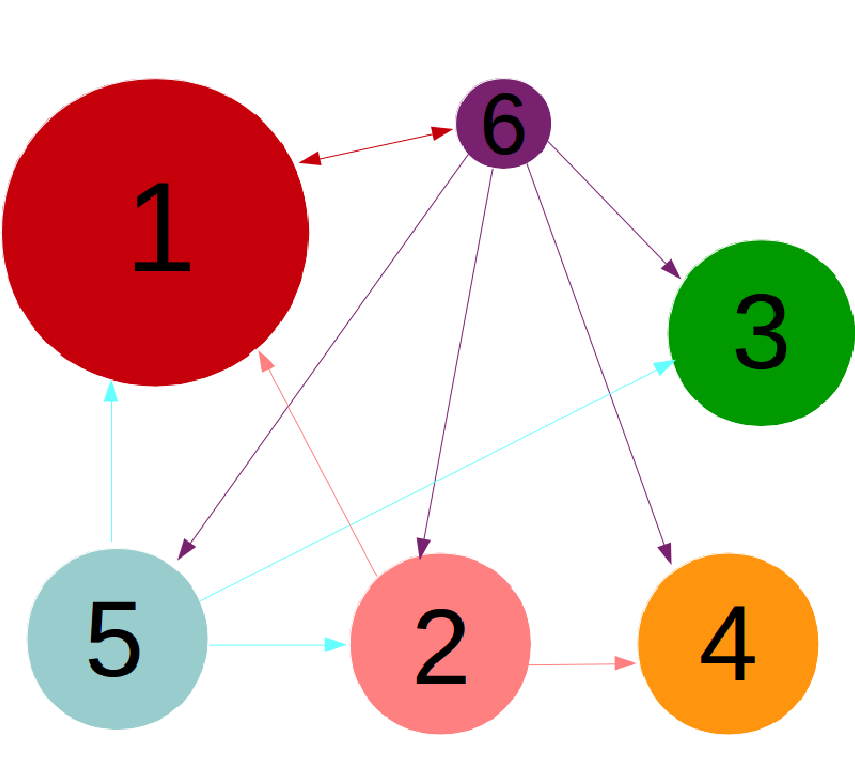
\includegraphics[width=7cm]{imagenes/liga2.png} \\
                      {\small Liga 2}
                    \end{center}
                \end{figure}


            En la liga 4 el equipo 1 gana con todos los que juega excepto cuando juega con el 6 que empata. El equipo 6 empata todos. El resto de los equipos quedan iguales que en la liga 2.

                \begin{figure}[h]
                    \begin{center}
                      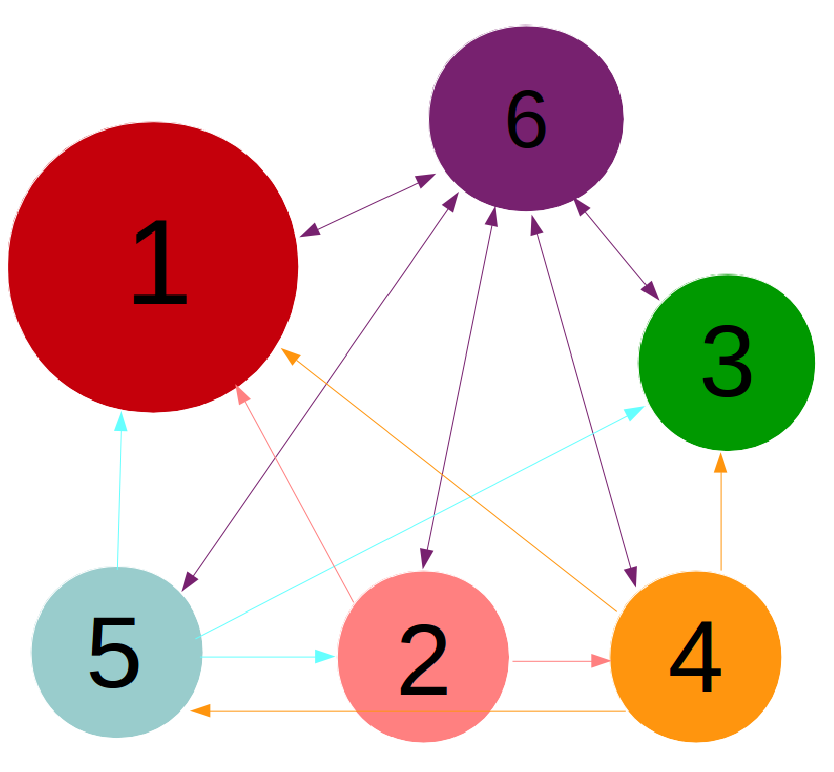
\includegraphics[width=7cm]{imagenes/liga4.png} \\
                      {\small Liga 4}
                    \end{center}
                \end{figure}

            Por último en la liga 5 el equipo 1 gana con todos los que juega excepto cuando juega con el 6 que empata. El equipo 6 empata todos. El equipo 3 pierde con todos los que juega excepto cuando juega contra el 6 que empata. El resto de los equipos quedan iguales que en la liga 2.

             \begin{figure}[h]
                \begin{center}
                  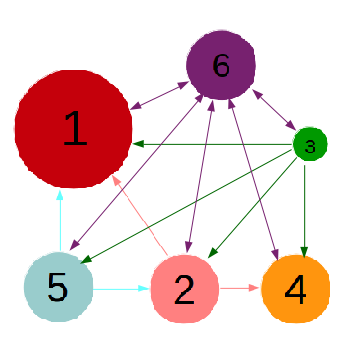
\includegraphics[width=7cm]{imagenes/liga5.png} \\
                  {\small Liga 5}
                \end{center}
            \end{figure}

            \subsubsection*{Hipótesis}
            Suponemos que en el método en el que se les da 0 puntos a los equipos empatados lo que va a pasar es que para dos equipos en los cuales uno empata todos los partidos en los que juega y otro que pierde (es indistinto si cuando juegan entre ellos empatan o pierde el primero) ambos quedarán con igual puntaje, lo que es injusto para el equipo que empata. Suponemos que esto se va a poder observar bien en la liga 5, ya que el equipo 3 pierde todos los partidos menos uno que lo empata (cuando juega contra el 6) y el 6 que empata todos. Ambos equipos quedarán últimos en el ranking final. Además si un equipo fuerte juega con uno débil y estos dos empatan entonces para ambos será lo mismo que no haber jugado, lo que no es justo para el equipa débil. Esto se puede ver en la liga 2 ya que el equipo 1 vence contra todos menos con el 6, con quien empata. El equipo 6 pierde con todos menos con el 1. En el resultado final el equipo 6 obtendrá 0 puntos a pesar de haber empatado con el equipo mas fuerte de la liga.

            En el método en el cual se le otorga una cantidad de puntos distinta de 0 al empate se supone que cuando un equipo débil le gane a uno fuerte va a subir mucho en el ranking. Esto es así ya que el peso que le da el enlace del equipo fuerte al débil es muy grande. Lo que va a pasar cuando estos equipos jueguen es que para el que lleva la delantera va a ser casi indistinto perder que empatar mientras que para el otro empatar lo favorece demasiado. Esto se puede observar en la liga 2. Suponemos que el equipo 6 (quien perdió todos menos uno que empató) quedará en una posición mucho mejor en el ranking por haber empatado con el 1 (quien gano todos los otros partidos que jugó). Además en este caso veremos que sucede con los rankings a medida que aumentamos el puntaje otorgado a los equipos que empatan. Suponemos que para valores muy grandes del empate puede pasar que sea mas conveniente empatar que ganar. Esto puede suceder ya que para determinar los puntos que se obtienen cuando se gana un partido hay que calcular la diferencia de goles. Si empatar otorga muchos puntos entonces posiblemente la diferencia de goles sea menor que lo que se puede obtener al empatar. Esto se puede observar en la liga 4. Suponemos que para valores de empate muy grandes el equipo 6 (quien empato todos) superará en el ranking final al equipo 1 (quien gano todos).

            En el tercer método, el valor de C2 representa la importancia que se le da a la matriz de empate. Suponemos que al aumentar este valor, cuando empaten dos equipos en los cuales uno sea débil y el otro fuerte, la cantidad de posiciones que ascenderá el equipo débil será mayor. Suponemos que con valores de C2 intermedios no ocurrirá que el equipo débil que empató con el fuerte ascienda demasiado en el ranking pero si se le otorgarán puntos por ello. Esto se puede observar en la liga 5 donde suponemos que se observará que empatar es mejor que perder pero peor que ganar y en la liga 2 donde el equipo 6 no va a tomar puna posición en el ranking muy elevada solo por haber vencido a un equipo fuerte pero tampoco quedará con cero puntos.

            \subsubsection*{Datos de entrada}
            Se tomará como valor de tolerancia 0.00001 y el valor de c 0.85. Se eligió el valor de la tolerancia y el de c arbitrariamente, procurando que los casos de prueba no fueran excesivamente grandes para no prolongar innecesariamente la duración de las pruebas. Las 3 ligas utilizadas se encuentran en la carpeta exp3-partidos. Los valores de puntajes que se les darán a los equipos que empaten que se pasarán como parámetro en el segundo método son 0, 1, 2, 3, 4, 5, 6, 7, 8, 9 y 10. Los valores de c que se pasarán para el tercer método serán 0.1, 0.15, 0.2, 0.25, 0.3, 0.35 y 0.4. Los valores de k y c que se observan en los gráficos son los valores más representativos.

            \subsubsection*{Resultados}
            \noindent{} \begin{minipage}{\textwidth}
                \begin{center}
                    \vspace{1em}

                    \begin{tabular}{cc}
                        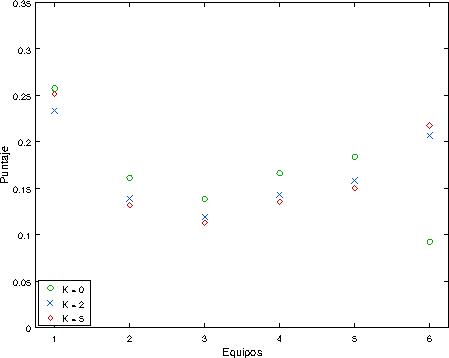
\includegraphics{graficos/exp3-partidos-liga2-K.pdf} & 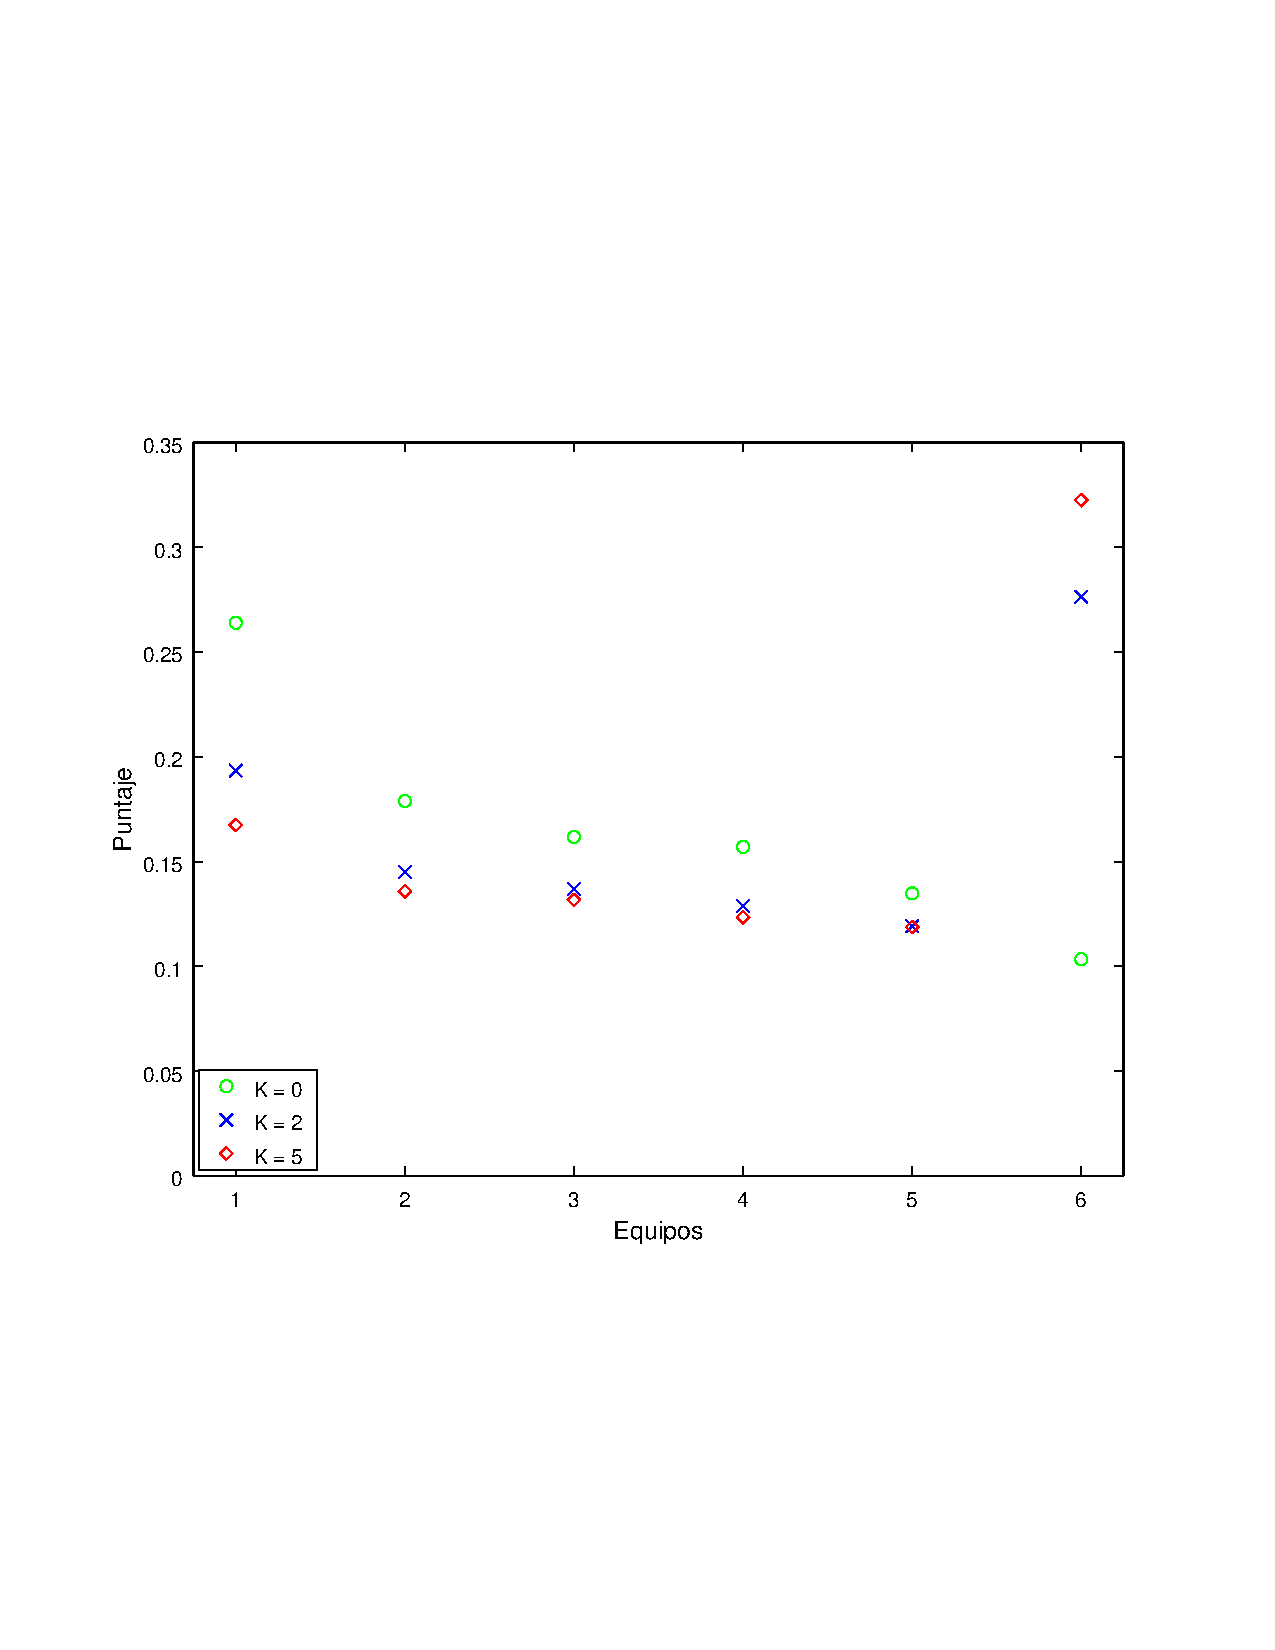
\includegraphics{graficos/exp3-partidos-liga4-K} \\
                        {\small Liga 2}                                      & {\small Liga 4}
                    \end{tabular}
                \end{center}
            \end{minipage}

            \noindent{} \begin{minipage}{\textwidth}
                \begin{center}
                    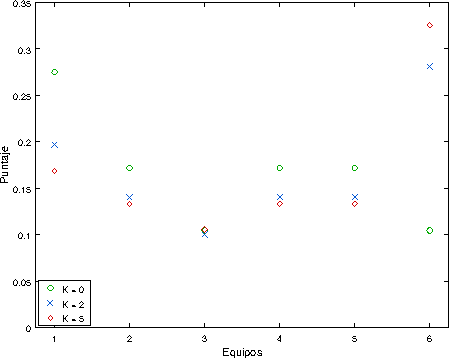
\includegraphics{graficos/exp3-partidos-liga5-K} \\
                    {\small Liga 5}

                    \vspace{1em}

                    Resultados arrojados por el experimento 2 para el método (2).

                    \vspace{1em}
                \end{center}
            \end{minipage}

            \noindent{} \begin{minipage}{\textwidth}
                \begin{center}
                    \vspace{1em}

                    \begin{tabular}{cc}
                        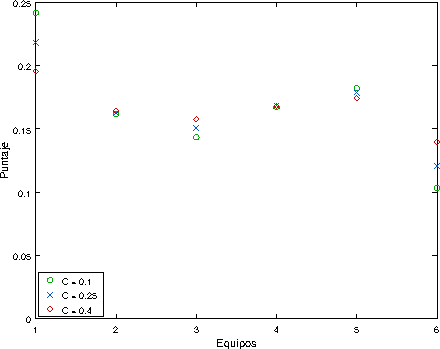
\includegraphics{graficos/exp3-partidos-liga2-C.pdf} & 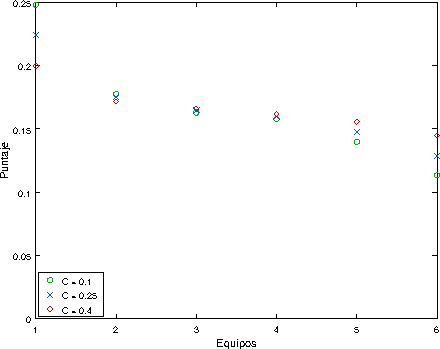
\includegraphics{graficos/exp3-partidos-liga4-C} \\
                        {\small Liga 2}                                      & {\small Liga 4}
                    \end{tabular}
                \end{center}
            \end{minipage}

            \noindent{} \begin{minipage}{\textwidth}
                \begin{center}
                    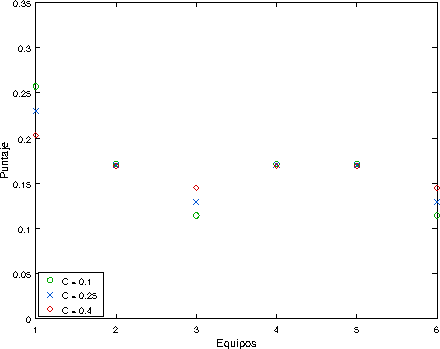
\includegraphics{graficos/exp3-partidos-liga5-C} \\
                    {\small Liga 5}

                    \vspace{1em}

                    Resultados arrojados por el experimento 2 para el método (3).

                    \vspace{1em}
                \end{center}
            \end{minipage}
        

            \subsubsection*{Discusión}
            Como se puede ver en el gráfico de la liga 2 modificando el k, el equipo 6 tiene muy poco puntaje cuando el k vale cero ya que al haber perdido todos y tener únicamente un empate, si éste vale cero entonces su puntaje es el mas bajo. Cuando el k aumenta, entonces se le dan puntos por el empate. Como este empate fue con un equipo fuerte entonces deja al equipo 6 muy bien posicionado en la tabla.

            En el gráfico de la liga 4 modificando k puede verse como a pesar de que el 1 ser el equipo con mas partidos ganados, al ponerle valores mas altos al puntaje que obtienen los equipos cuando empatan que la diferencia de goles que tiene el equipo mas fuerte, entonces el que empato logra tomar posiciones más altas en la tabla.

            En el gráfico de la liga 5 modificando k puede observarse cuando el k vale 0 que los equipos 3 y 6 quedan empatados a pesar de que uno haya perdido en todos y el otro empatado. En cambio cuando se le da puntos a los equipos que empatan el equipo 6 sube mucho en el ranking. Incluso llega a superar al equipo que gano todos los partidos. Dejamos a experimentos futuros determinar cuál es el valor que deberá tomar k para que no suceda que supere al equipo vencedor.
            
            Cuando usamos el método 3, al que le pasamos por parámetro un C2 que será el nivel de importancia que se le da a la matriz de empate explicada anteriormente, podemos observar que los puntajes que obtienen los equipos que empatan y los que pierden es exactamente el mismo, por lo tanto este método no cumple con el objetivo de lograr que un equipo que empata todos los partidos tenga mejor posición en el ranking que aquel que pierde pero que al mismo tiempo empatar contra un equipo fuerte no genere que el otro ascienda mucho en la tabla de posiciones. Además se puede ver que para los diferentes valores de C2 lo único que se modifica es el puntaje de los equipos sin alterar el ranking. Cuando el C2 toma valores mas grandes se les asigna mayor puntaje a los equipos que empataron, dejando con menos puntos a los que ganaron. 

            También se puede observar que para los equipos que no empatan con ninguno, la variación del C2 no les afecta. Esto es así ya que el C2 sólo modifica la matriz de empates. En el caso de los equipos que no empataron nunca el valor correspondiente de la matriz para ellos es cero. Al multiplicarlo por el C2 sigue siendo cero. Entonces ésta variación no modifica su puntaje.

            Concluimos que el criterio mas acertado de los que analizamos hasta el momento es otorgarle al empate una determinada cantidad de puntos sin que genere que empatar se mejor que ganar pero que tampoco suceda que si un equipo fuerte juega contra uno débil y empatan éste ultimo obtenga cero puntos. 
